\graphicspath{{Ch4_Jets/figures/}}

\chapter{Jets}
As discussed in Section~\ref{sec:monte_carlo}, partons created during $pp$ collisions undergo a showering process where they produce cascades of additional strongly interacting particles through gluon radiation and splitting.
As this showering process concludes and the products approach a sufficiently low energy ($\approx 1$ GeV) the resulting partons hadronize and produce a spray of colorless hadrons called a ``jet'' which interacts with both the tracking and calorimeter systems of the ATLAS detector.
Jets are reconstructed by employing \textit{jet clustering algorithms} which take a set of constituent inputs from the event and combine them to output a set of jets.
At the ATLAS experiment jets may be constructed using only tracks as inputs, only calorimeter clusters and inputs, or a combination of both.

%TODO: basic jet cartoon figure

Due to their aggregate nature, the notion of a \textit{jet} is not as immediately or clearly interpreted as are other physics objects such as electrons, muons, and photons.
This allows for a significant amount freedom in how jets are defined and reconstructed in collider experiments.
Furthermore the manner in which individual constituents are combined, and the characteristic size of the resulting jets (in the $\eta$-$\phi$ plane) can be altered on a per-algorithm basis.
To deal with this ambiguity a set of properties that must be met by any standardized jet definition were outlined in December of 1990 \cite{Huth:217490} as follows:
\begin{enumerate}
    \itemsep0em 
    \item Simple to implement in an experimental analysis.
    \item Simple to implement in a theoretical calculation.
    \item Defined at any order of QCD perturbation theory.
    \item Yield finite cross section at any order of perturbation theory.
    \item Yield a cross section that is \textit{relatively} insensitive to hadronization.
\end{enumerate}
This set of rules allows for better communication between experimental and theoretical physics results, as well as better comparison of results between different collider experiments.

\section{Jet Constituents}

All jet clustering algorithms take as input a set of four-vectors representing all the products of parton showering and hadronization, known as \textit{constituents}.
These constituents compose \textit{all} the potential jets in the event, and it is the job of the jet clustering algorithm to convert these to a set of four-vectors representing only the corresponding jets from the event.
These constituents can be created with information from any particular ATLAS sub-detector or combination thereof, as long as they encode the four-vectors of the particles produced during the jet showering/hadronization process.
The most relevant constituent types for this analysis are outlined below.

\subsection{Calorimeter Clusters}
The information quality contained within a collection of calorimeter signals of a given collision event can be increased by grouping the signals into \textit{topologically connected cell clusters}.
This strategy helps to reduce the impact of background electronic noise and other sources of calorimeter fluctuation such as the presence of pile-up.
The finely segmented lateral ($\eta$-$\phi$) readout together with the longitudinal sampling layers allows the ATLAS calorimeter system to resolve spatial signal patterns important for jet reconstruction while efficiently removing insignificant signals caused by noise.

\newcommand{\LCTopoSig}{\ensuremath{\varsigma^{\mathrm{EM}}_{\mathrm{cell}}}}
These topo-clusters are formed by a growing-volume algorithm \cite{Aad:2016upy} which begins with a calorimeter cell possessing a highly significant \textit{seed signal}, where significance is defined as the ratio of the cell signal magnitude over the expected noise:
\begin{equation}
    \LCTopoSig = \frac{E^{\mathrm{EM}}_{\mathrm{cell}}}{\sigma^{\mathrm{EM}}_{\mathrm{noise,cell}}}
    \label{eqn:lctopo_sig}
\end{equation}
The growth of the topo-cluster proceeds iteratively by connecting nearby cells, where the seeding, growth, and boundary conditions are controlled by placing bounds on the cell significance (Eq.~\ref{eqn:lctopo_sig}), as shown in Figure~\ref{fig:lctopo_formation}.
The four-vector corresponding to each topo-cluster is computed by a weighted combination of all cells contained in the topo-cluster.
The weights are necessary because each cell is allowed to contribute (unevenly) its energy to two separate topo-clusters.

\begin{figure}
	\centering
	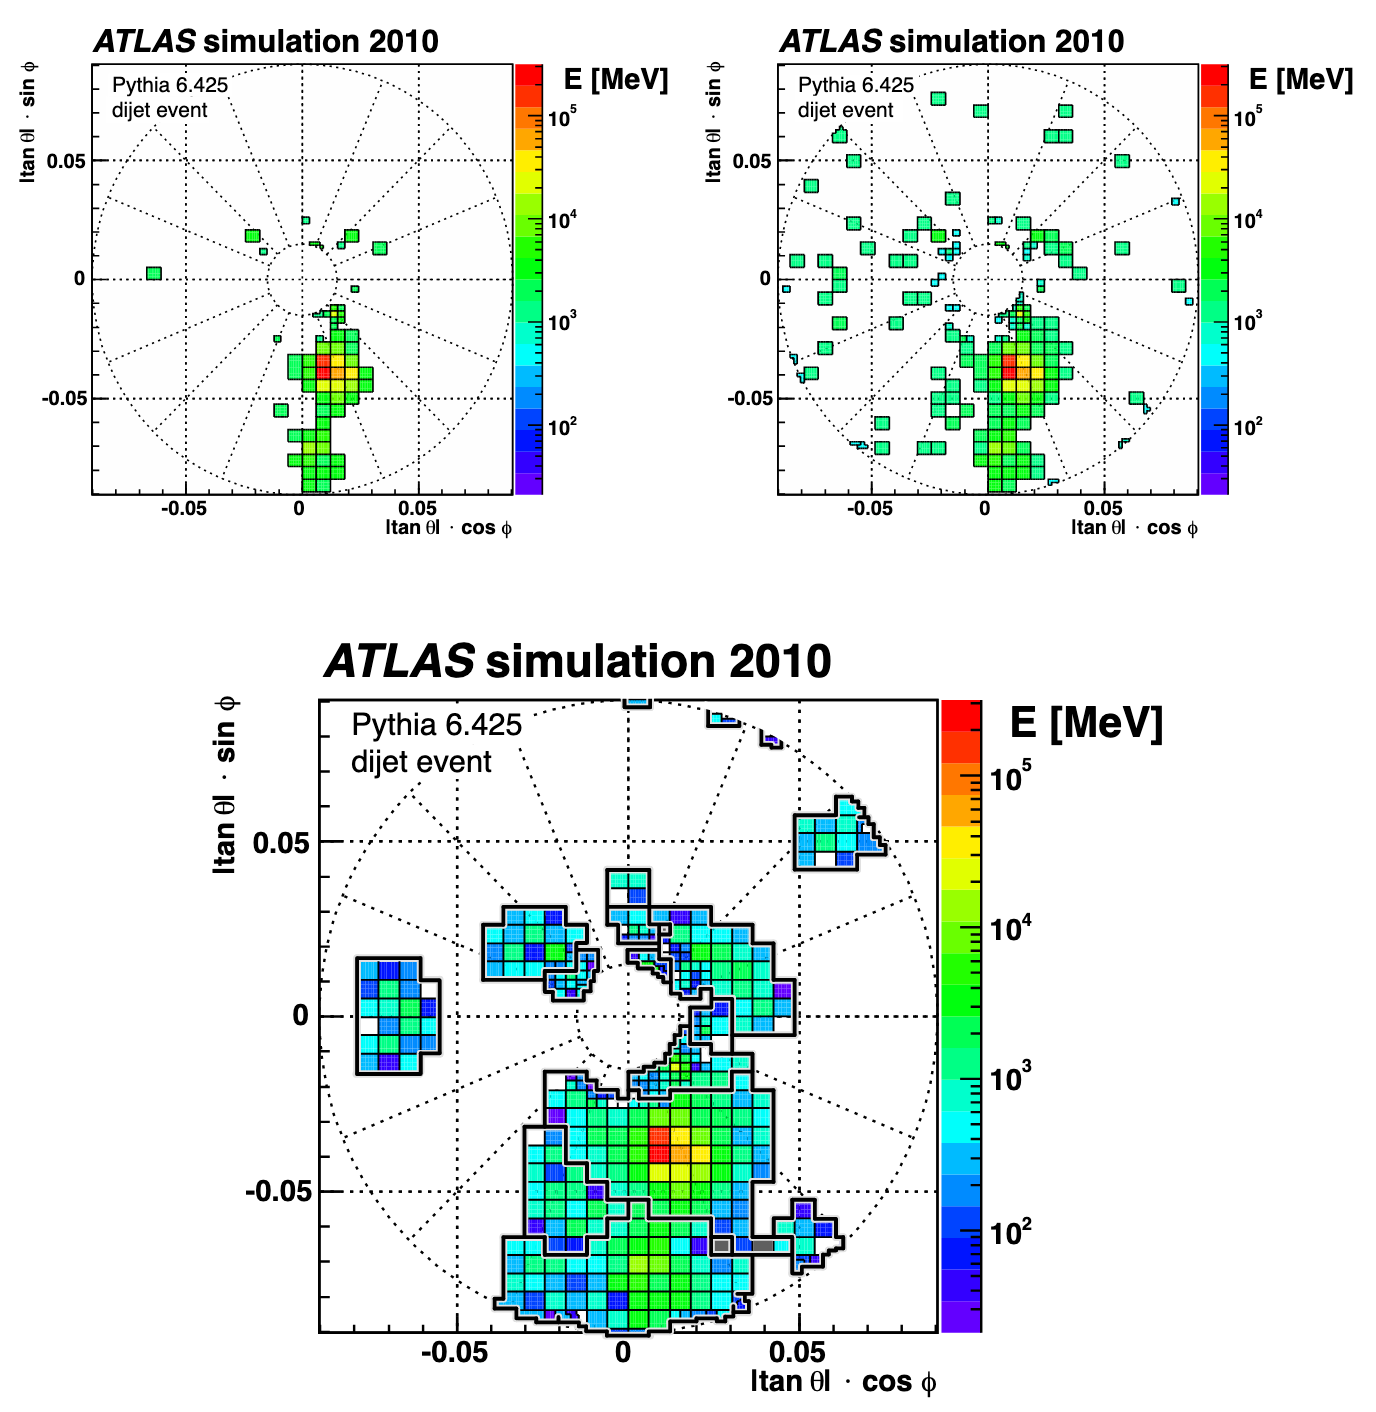
\includegraphics[width=\textwidth]{lctopo_formation}
	\caption{
	Stages of topo-cluster formation in the FCAL calorimeter for a simulated dijet event.
	Cells with $\LCTopoSig > 4$ (top left) are used in the seeding, cells with $\LCTopoSig > 2$ (top right) control the topo-cluster growth.
	The final set of topo-clusters (bottom) is shown with black outlines around each cluster.
	Adapted from \cite{Aad:2016upy}.
	}
	\label{fig:lctopo_formation}
\end{figure}

\subsection{Tracks}
\cite{ATLAS-CONF-2016-035}

\dots

\subsection{Track-Calo Clusters}
\cite{ATL-PHYS-PUB-2017-015}
\dots

\section{Clustering Algorithms}
\dots

\subsection{Anti-$k_t$}
\cite{Cacciari:2008gp}
\dots

\subsection{Variable Radius (VR)}
\cite{ATL-PHYS-PUB-2017-010}
\dots

\section{Trimming/Grooming}
\cite{ATLAS-CONF-2012-065}
\dots

\section{Jet Substructure}
\dots

\subsection{Jet Mass}
\dots
\subsection{Jet \Dtwo}
\dots

\section{B-Jet Identification}
\dots